\section{Data And Methodology}
\label{sec:data_and_methodology}

Given the large number of sociological reasons why broadband should impact
economic growth in theory, it seems that we should be able to quantitatively
measure the actual impact over the decade of broadband's use. The largest study I
know of that performed such an analysis on a large scale,
the World Bank study~\cite{qiang2009economic}, used data from 2007.
In this section I describe the data sources used in that study in detail,
cover my own use of those same data sources including preprocessing and sanity
checks, and describe the methodology I used to corroborate and update
the World Bank's result.

\subsection{Data Sources}

The data from Quiang et. al's study came from two sources:
\begin{enumerate}
\item The International Telecommunication Union World Telecommunication Indicators
Database~\cite{itu} provides data on communications technology in over 200
developed and developing regions. The specific metrics used for this study
include mobile and cellular telephone subscriptions, overall fraction of the
popultion using the Internet, and broadband penetration numbers, dating from
2001-2011.
\item The World Bank World Development Indicators Online Database~\cite{wdi}
maintains over 1,500 metrics ranging from GDP to number of acres used for
forestation across over 200 countries. We rely on this database for GDP, primary school enrollment
rates, and investment share from 1980-2011.
\end{enumerate}

The two databases differed in some ways, so I needed to perform some
preprocessing on the data to make it useable. For example, I enumerated all
country names, and converted all names to a canonacal format so that the
datapoints could be matched up programatically between the two sources. In
cases of ambiguity in which specific metrics Quiang et al. used for their
analysis (e.g. raw GDP versus GDP adjusted for PPP), I experimented with the
output to ensure that it closely matched Qiang's final results.

I also relied on country classifications from the World
Bank~\cite{classifications}
to bucket countries into high, low and middle income countries.
These metrics were used as dummy variables in the regression
analysis, described below.

\subsection{Methodology}

Econometric regression over 6 variables.
Across 120 countries.
Bucketed into low/middle/high income.

Dependent variable: GDP.

Independent variables:
\begin{enumerate}
\item Average broadband penetration per 100 people.
\item GDP per capita in 1980.
\item Ratio of gross investment to GDP.
\item Primary school enrollment (human capital).
\item Dummy variable for countries in Sub-Saharan Africa
\item Dummy variable for countries in Latin America / Caribbean
\end{enumerate}

These variables were chosen based on an Endogenous Growth Model.
Explain all the things I learned about growth models (why I didn't use an
exogenous model, etc.). The variables used in this regression are plotted over time
in figure~\ref{fig:variables}.

Fancy math equation for endogenous growth.

The code used to perform this analysis is publicly available~\cite{github}.

\begin{figure}[!ht]
\label{fig:variables}
\begin{center}
\caption{Variables Used in Regression}
\subfigure[]{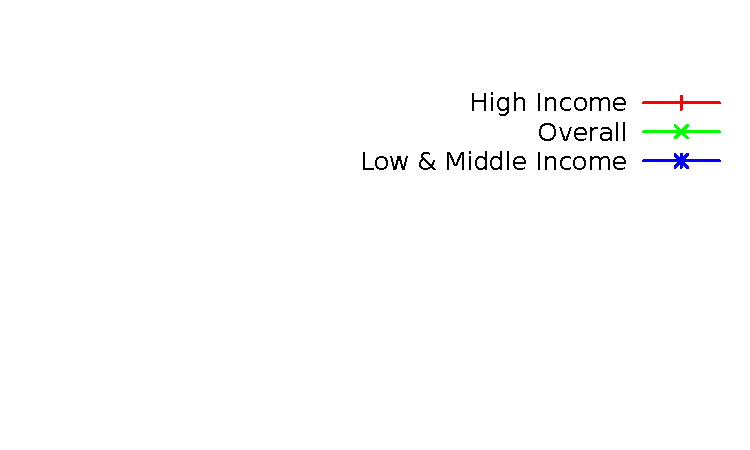
\includegraphics[width=0.49\textwidth]{images/key.pdf}}
\subfigure[]{\centering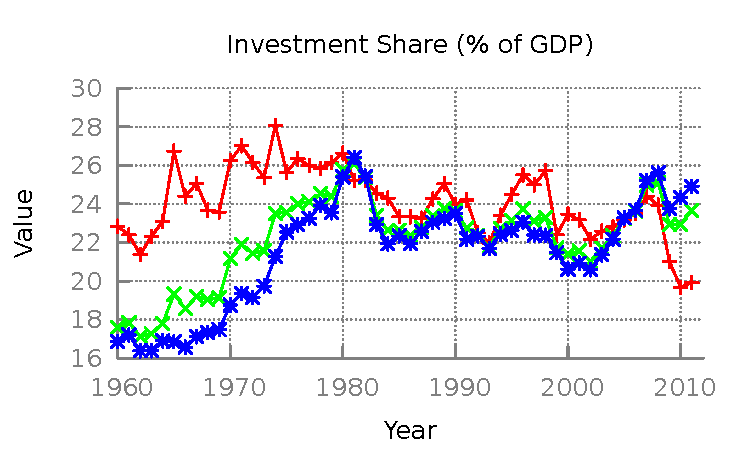
\includegraphics[width=0.45\textwidth]{images/NE_GDI_TOTL_ZS.pdf}}
\subfigure[]{\centering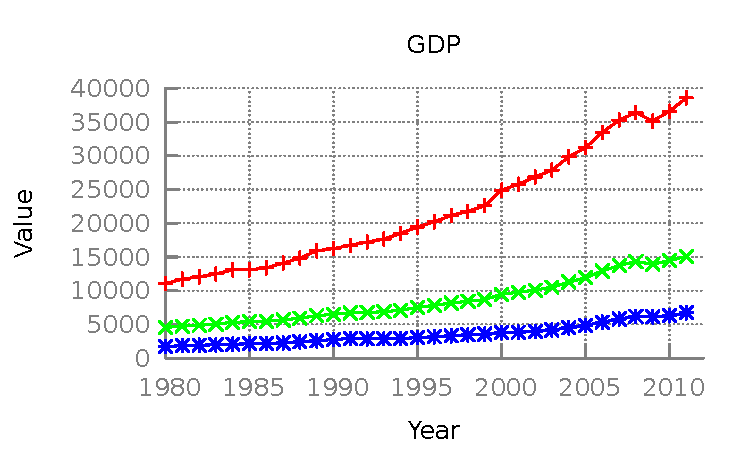
\includegraphics[width=0.45\textwidth]{images/NY_GDP_PCAP_PP_CD.pdf}}
\subfigure[]{\centering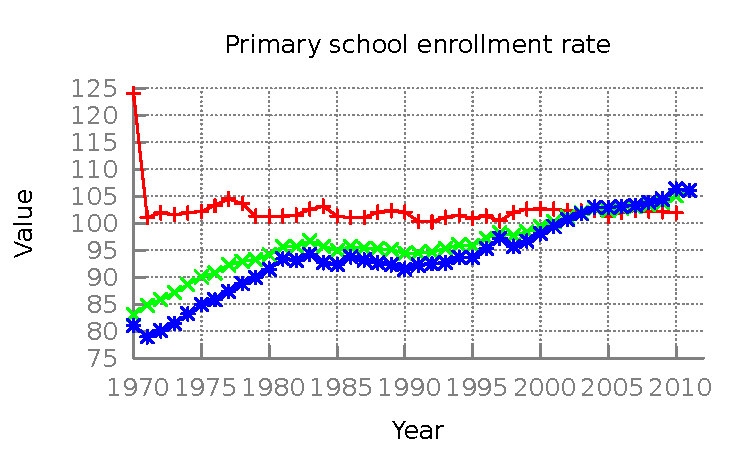
\includegraphics[width=0.45\textwidth]{images/SE_PRM_ENRR.pdf}}
\subfigure[]{\centering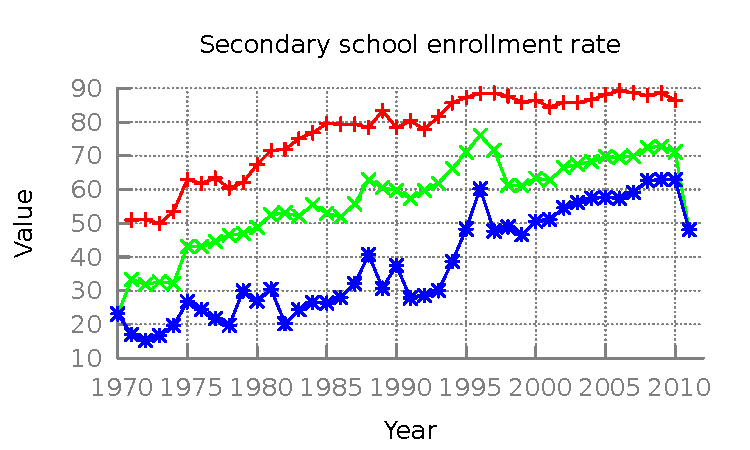
\includegraphics[width=0.45\textwidth]{images/SE_SEC_NENR.pdf}}
\subfigure[]{\centering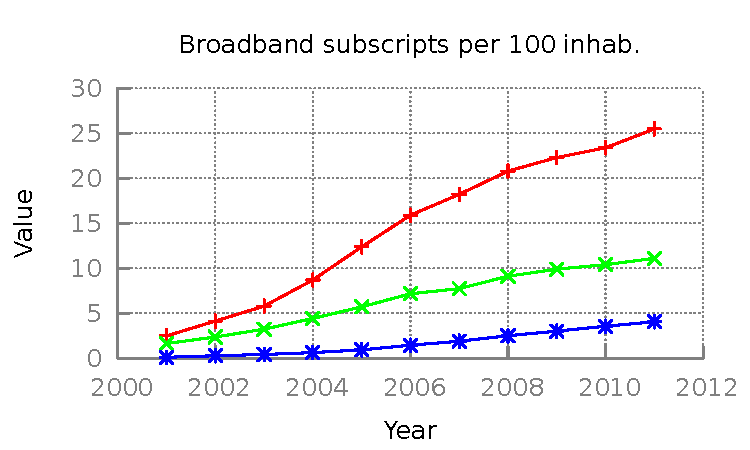
\includegraphics[width=0.45\textwidth]{images/broadband_per_100.pdf}}
\subfigure[]{\centering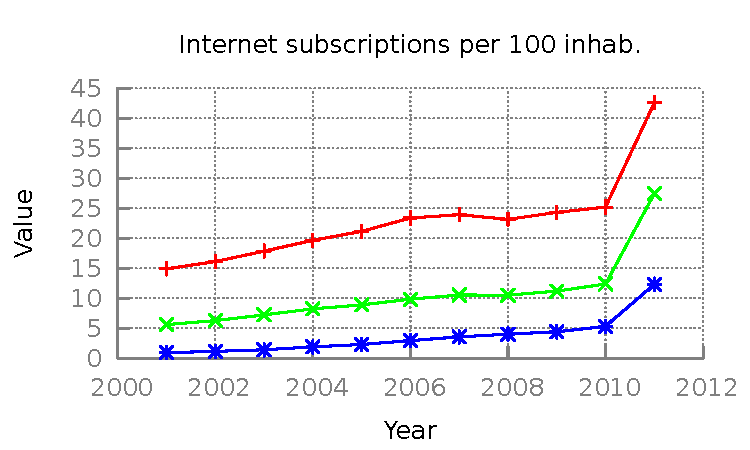
\includegraphics[width=0.45\textwidth]{images/inet_per_100.pdf}}
\subfigure[]{\centering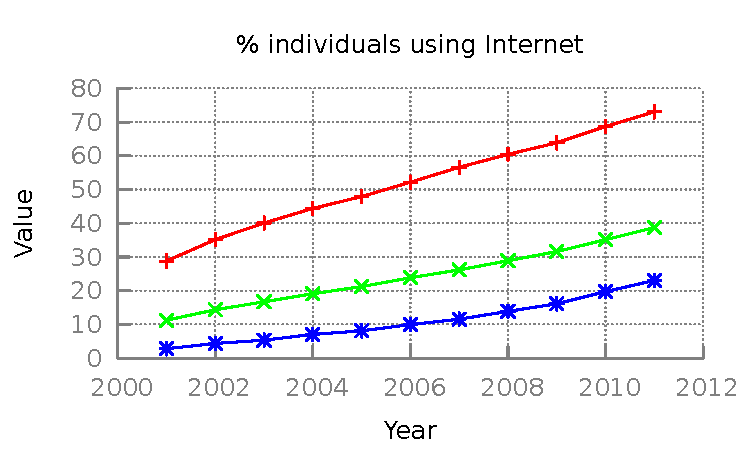
\includegraphics[width=0.45\textwidth]{images/inet_percent.pdf}}
\subfigure[]{\centering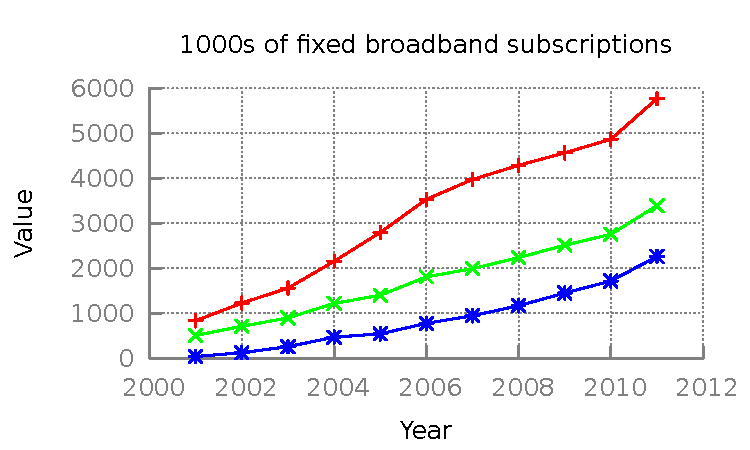
\includegraphics[width=0.45\textwidth]{images/total_broadband.pdf}}
\subfigure[]{\centering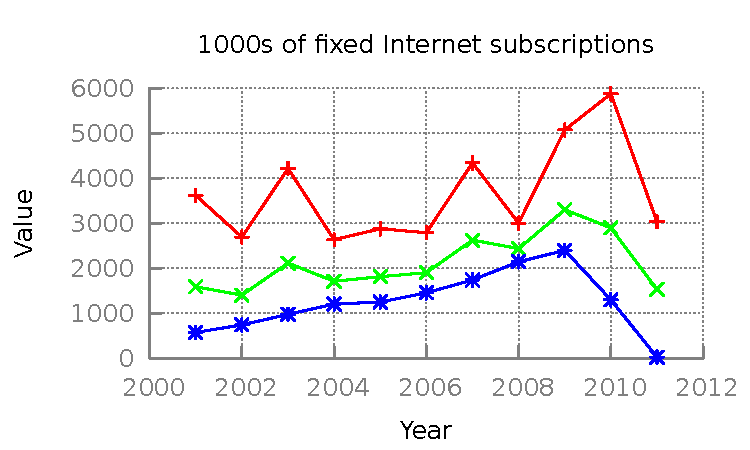
\includegraphics[width=0.45\textwidth]{images/total_inet.pdf}}
\end{center}

\end{figure}
